\chapter{Applications to Probabilistic Aerodynamic Databases for Full Aircraft} \label{sec:results}

Given these building blocks, this section highlights their application to a real-world engineering problem. For this purpose, the development of a multi-fidelity probabilistic aerodynamic database for the NASA CRM aircraft is shown. It combines numerical analyses of different fidelities (vortex lattice and RANS), experimental data from wind-tunnel observations, and their associated uncertainties (provided by SMEs, the RANS UQ methodology, and experimental data uncertainties, respectively). The result is a probabilistic database that is valid within the operating envelope of the aircraft. In addition to providing mean predictions for the forces and moments that would be experienced by the aircraft under different operating conditions, this database provides variance information about the uncertainty in the predictions. 

The NASA CRM is a well-investigated full-configuration aircraft \cite{rivers_further_2012,rivers_experimental_2010} that was developed with the goal of creating a baseline geometry upon which numerous experimental and computational studies could be performed and compared \cite{morrison20094th,levy2013summary,morrison20166th,roy2017summary,tinoco2017summary}. The wealth of experimental and computational data lends itself well for the purpose of showcasing the performance of the uncertainty quantification and multi-fidelity data fusion techniques laid out in Section \ref{sec:methodology}. 

\section{Uncertainty Quantification in RANS CFD} \label{sec:crm_uq}
While the eigenspace perturbation methodology has been demonstrated on a variety of test cases, this is its first application on a full-configuration aircraft. The full aircraft configuration is identical (without accounting for aeroelastic deflections of the model) to the one that was tested in the wind tunnel and corresponds closely to a Boeing 777 aircraft with a fully-redesigned wing. The transonic simulation conditions are described in Table \ref{NASA_CRM_test_cond}. Note that the range of angles of attack, at a free stream Mach number of 0.85, lead to non-linear physical phenomena and flow separation that can greatly increase the uncertainties in the RANS predictions. Separated flow exists for $\alpha > 4^\circ$ at this Mach number. All of the necessary RANS CFD simulations were conducted using the SU2~\cite{su2_aiaajournal} solver. The SST turbulence model~\cite{menter1994two,menter2003ten} was used and the previously defined perturbations, Equations \eqref{equ:eigenvalue_pert} - \eqref{equ:vmin_vmax}, were applied to it. 

\begin{table}
\centering
    \captionsetup{justification=centering}
    \caption{Simulation conditions for the NASA CRM.} 
    \begin{tabular}{|c|c|}
        \hline
        Mach Number & $0.85$ \\ \hline
        Reynolds Number & $5\times10^6$ \\ \hline
        Reference chord length & $7.00532$ m \\ \hline
        Freestream Temperature & $310.928~\text{K}$ \\ \hline
        $\alpha$ & $-2^\circ \leq \alpha \leq 12^\circ$ \\ \hline 
        $N$ (mesh elements) &  $11.8\times10^6$ \\ \hline
    \end{tabular}
    \label{NASA_CRM_test_cond}
\end{table}

Figure \ref{fig:crm_mesh} shows details of the unstructured mesh that was used for the CFD simulations. The computational domain is made of $11.8\times10^6$ mixed elements ($4.6\times10^6$ nodes) which corresponds to a coarse mesh based on the grid convergence studies performed for multiple solvers and grid topologies \cite{vassberg_summary_2010}. Figure \ref{fig:dpw4_alpha_sweep} presents results of the angle-of-attack sweep study from SU2 on the coarse mesh alongside results from comparable unstructured solvers, BCFD \cite{winkler_dorgan_cary_mani_2009} and FUN3D \cite{lee-rausch_application_2014} on their medium-sized meshes. 
The difference between the grid-converged drag at a fixed $C_L$ of 0.5 and the present study is approximately $4\%$; this difference can be used as a rough metric for the discretization uncertainty. This uncertainty could be reduced through additional grid resolution studies but is not considered a primary factor for the present demonstration.

\begin{figure}
    \centering
    \begin{subfigure}[Surface mesh of the NASA CRM.] {
        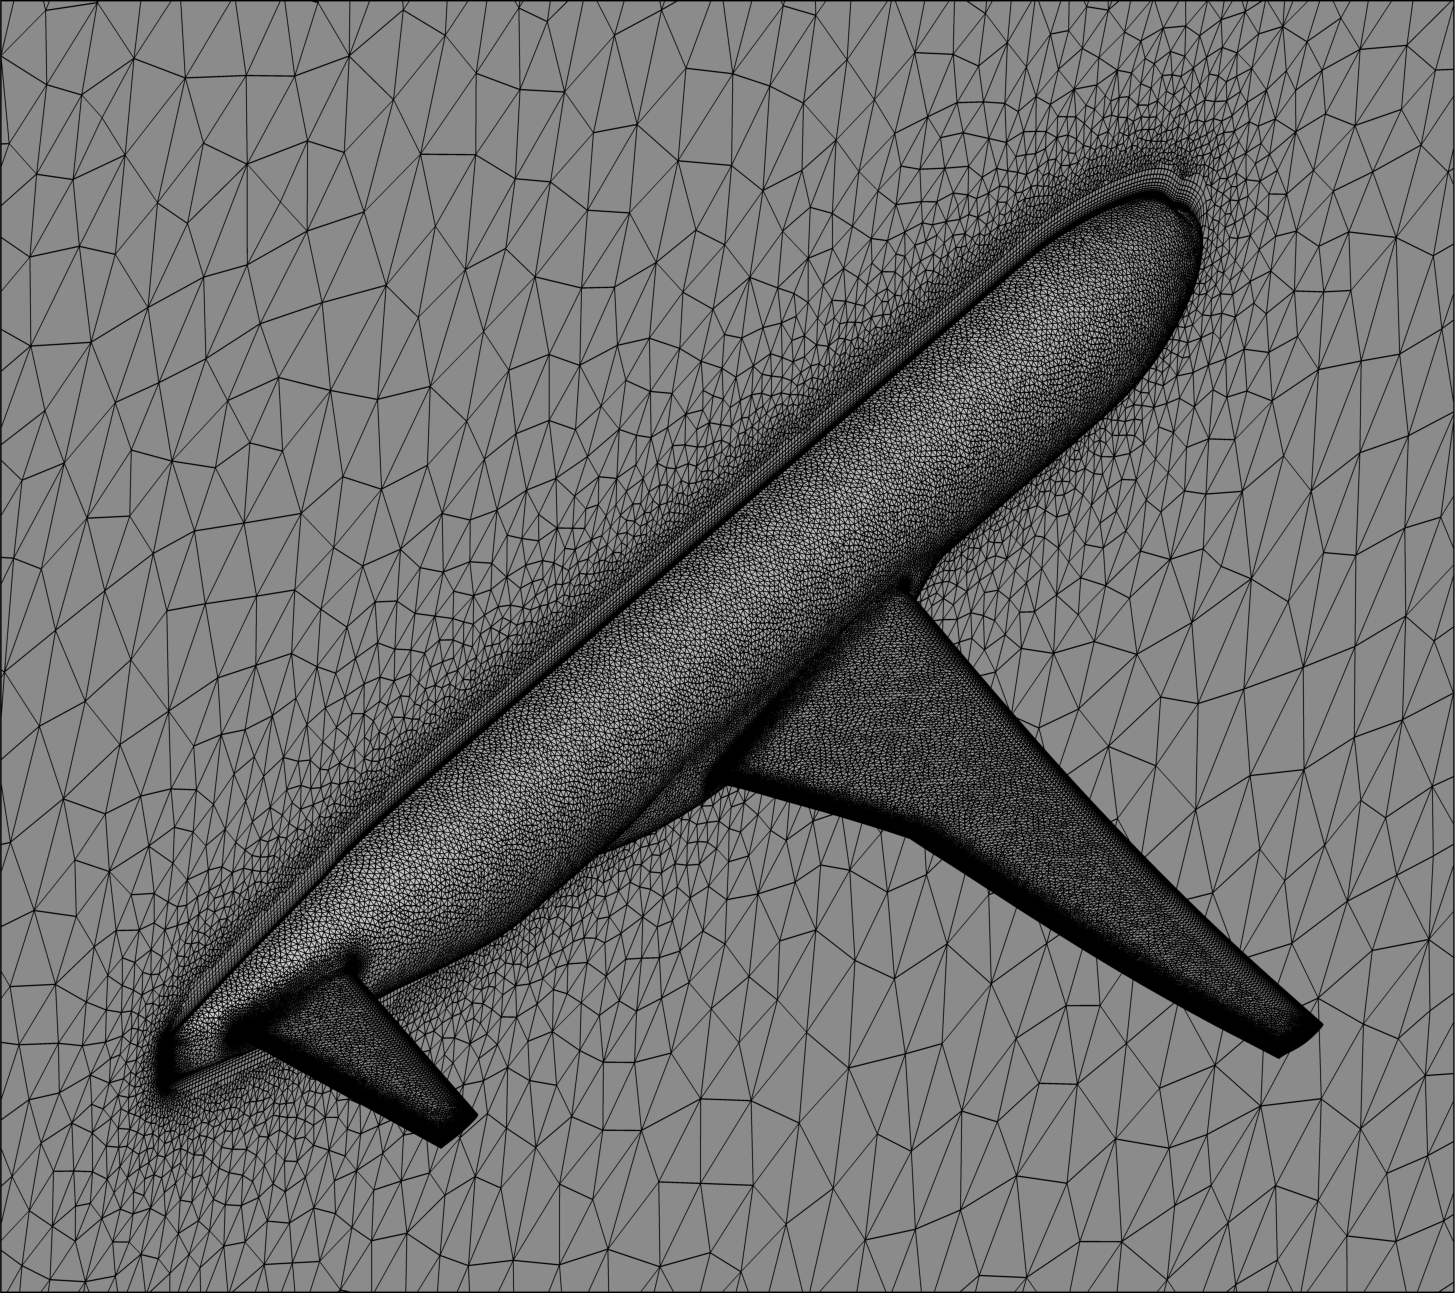
\includegraphics[trim=80 130 100 160, clip, width=.47\textwidth]{images/surface_mesh+symm.png} }
    \end{subfigure}
    \hfill
    \begin{subfigure}[Close up of the nose cone showing boundary layer cells on the symmetry plane.]{
        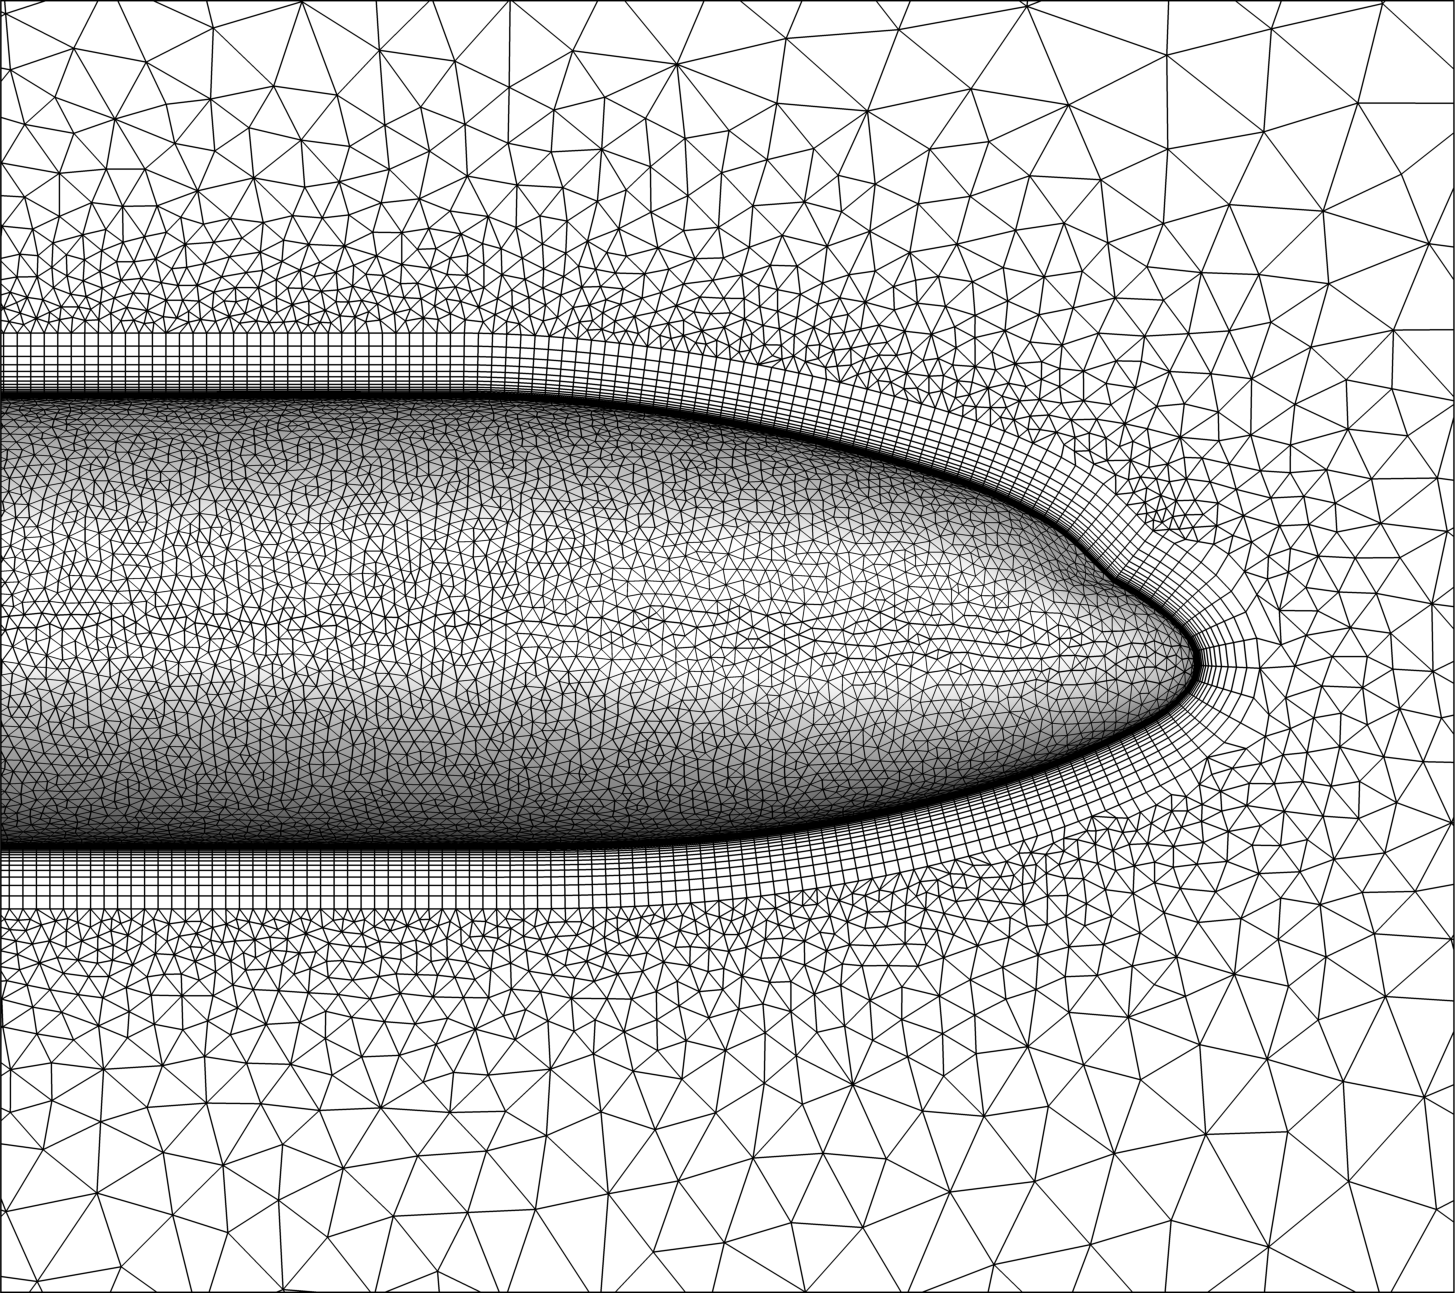
\includegraphics[trim=80 130 100 160, clip, width=.47\textwidth]{images/nose_side_view.png} 
    }
    \end{subfigure}
    \hfill
    \begin{subfigure}[Details of the wing surface mesh.]{
        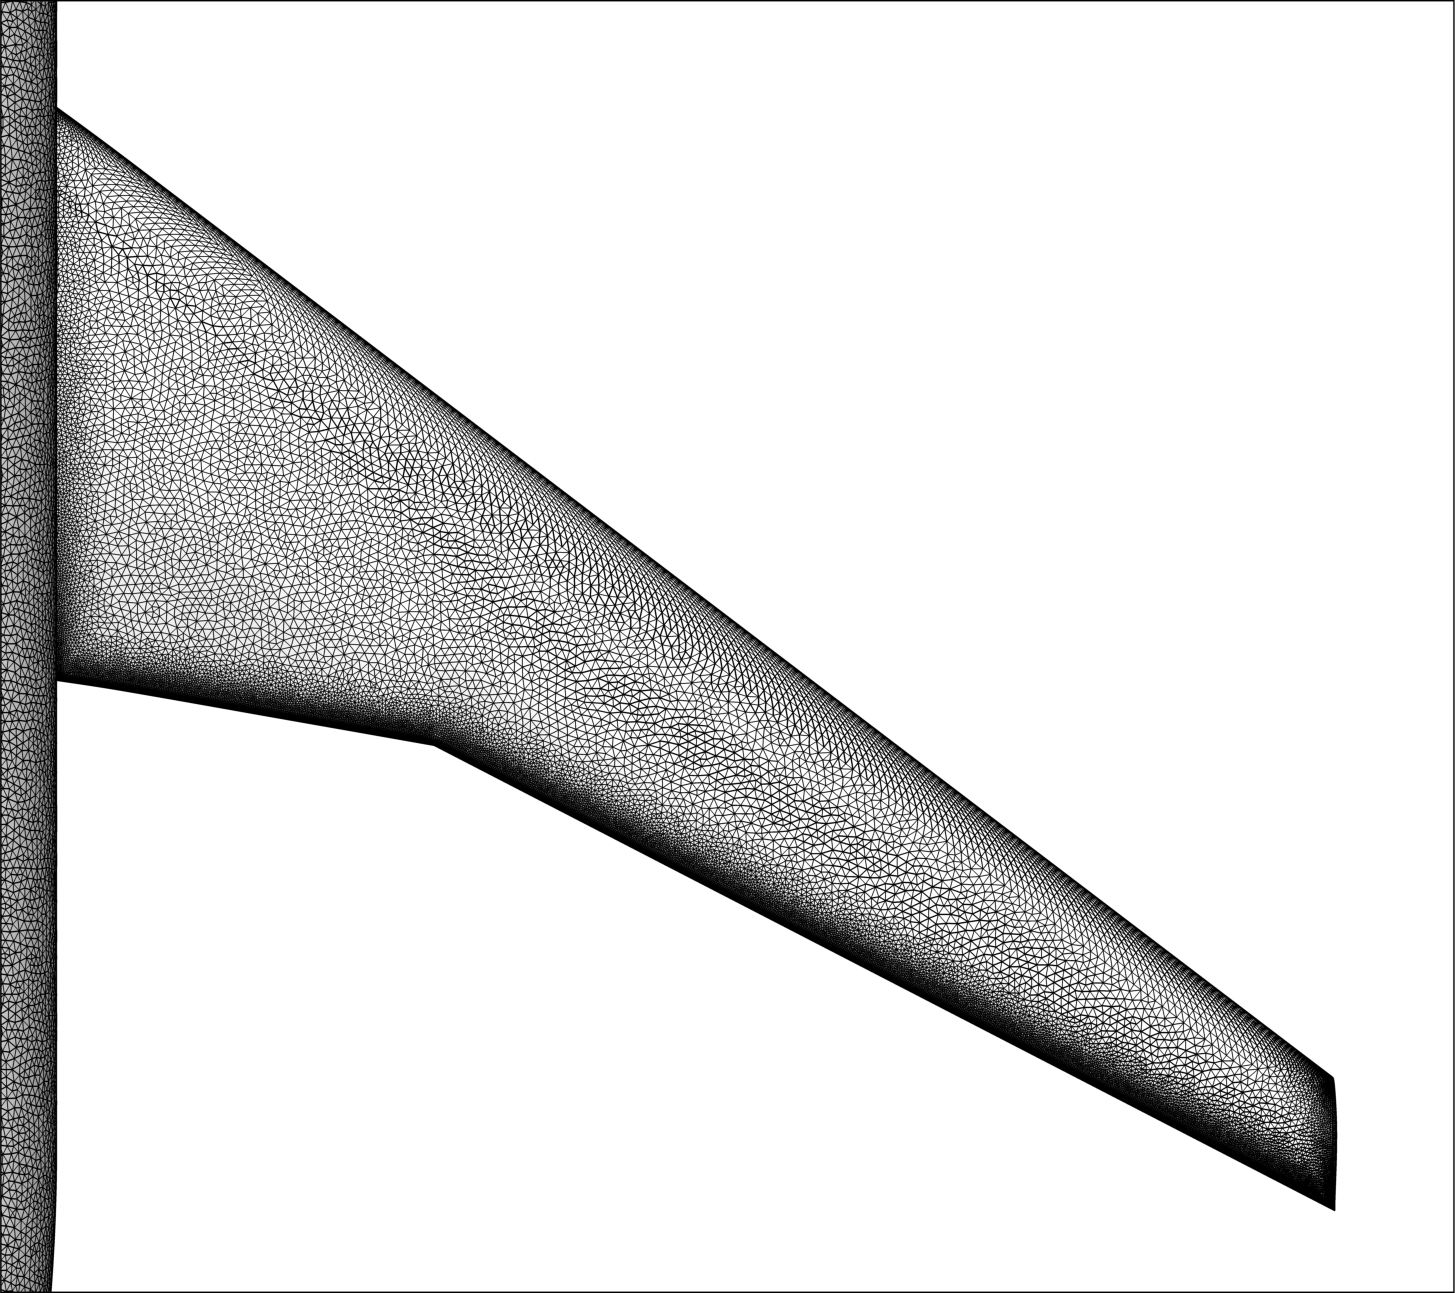
\includegraphics[trim=80 80 80 100, clip, width=.5\textwidth]{images/wing.png} 
    }
    \end{subfigure}
    \caption{Images of the NASA CRM mesh that was used for the CFD simulations.\label{fig:crm_mesh}}
\end{figure}

\begin{figure}{
\centering
    \includegraphics[width=.68\textwidth]{images/dpw4_alpha_sweep.eps} 
    \caption{Angle of attack sweep results from SU2 compared to other similar solvers. \label{fig:dpw4_alpha_sweep}}
    \hfill
}
\end{figure}


The convergence history for the the simulations required to characterize the uncertainty at a particular operating condition ($\alpha = 2.35^\circ$) is shown in Figure \ref{fig:convergence_history}. Most cases achieve 6 orders of magnitude reduction in the density residual. For the $1C, v_{max}$ case, the residuals stall but the solution is said to be converged once the force coefficients stabilize to 6 orders of magnitude (less than $10^{-6}$ change in force coefficients over $100$ non-linear iterations).

\begin{figure}{
\centering
    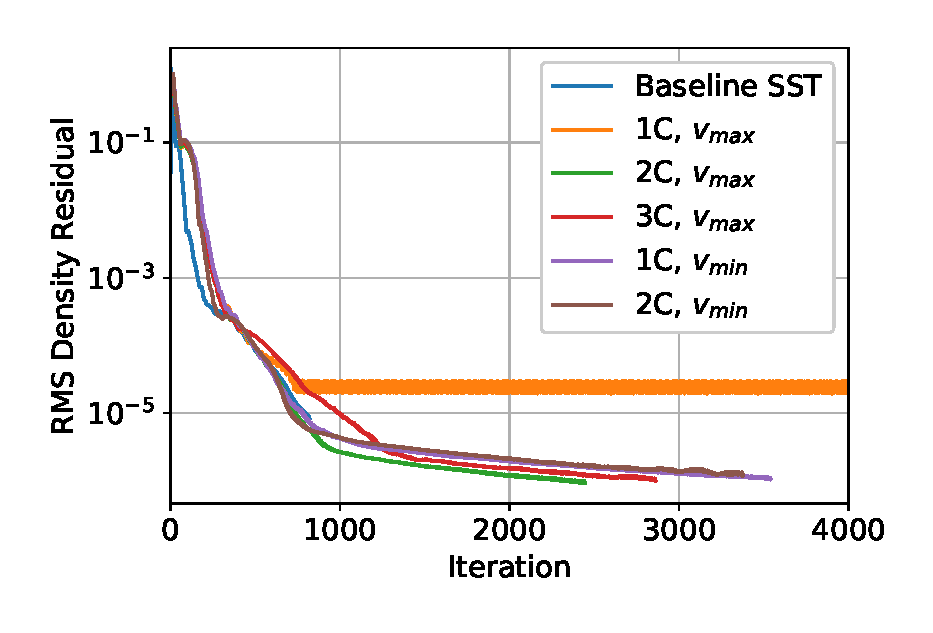
\includegraphics[trim=0 0 0 0, clip, width=.7\textwidth]{images/convergence_history.eps} 
    \caption{Convergence history of the density residual for RANS UQ CFD simulations at $\alpha = 2.35^\circ$, Baseline SST turbulence model + $5$ perturbed simulations. \label{fig:convergence_history}}
    \hfill
}
\end{figure}

In Figure \ref{fig:crm_su2_uq}, the results of these simulations are compared to wind tunnel data from the NASA Ames 11ft Wind Tunnel experiment \cite{rivers_experimental_2010}. In this figure, the solid black line represents the predictions made by the baseline SST turbulence model, the grey area represents the interval bounds predicted by the eigenspace methodology, and the black crosses represent the wind tunnel data. These wind tunnel data points have error bars associated with them but these are barely discernible on the scale of the plot. 

The performance of the UQ module is illustrated by comparing the variation of the coefficients of lift ($C_L$), drag ($C_D$), and longitudinal pitching moment ($C_m$) with respect to angle of attack ($\alpha$), as predicted by the CFD simulations to those experimentally determined. We start with $C_L$ vs. $\alpha$ in Figure \ref{fig:cl_vs_alpha}. At low angles of attack, the flow remains well attached to the aircraft body; therefore, the turbulence model does not introduce significant uncertainty in its predictions. Accordingly, the interval bounds predicted by the UQ module are relatively small. At higher angles of attack when there is flow separation over portions of the aircraft, turbulence models struggle to make accurate flow predictions due to the unsteady nature of the flow features and the structural limitations of the isotropic eddy viscosity enforced by the Boussinesq assumption. This is reflected in the growing uncertainty bounds predicted by the module. This overall trend is seen in all of the plots in Figure \ref{fig:crm_su2_uq}. 

\begin{figure}
    \centering
    \begin{subfigure}[$C_L$ vs. $\alpha$.] {
        \label{fig:cl_vs_alpha}
        \includegraphics[width=.45\textwidth]{images/cl_su2_uq.eps} 
    }
    \end{subfigure}
    \hfill
    \begin{subfigure}[$C_D$ vs. $\alpha$.]{
        \label{fig:cd_vs_alpha}
        \includegraphics[width=.45\textwidth]{images/cd_su2_uq.eps} 
    }
    \end{subfigure}
    \hfill
    \begin{subfigure}[$C_m$ vs. $\alpha$.]{
        \label{fig:cm_vs_alpha}
        \includegraphics[trim=4 0 0 0, clip,width=.45\textwidth]{images/cm_su2_uq.eps} 
    }
    \end{subfigure}
    \hfill
    \begin{subfigure}[$C_L$ vs. $C_D$.]{
        \label{fig:cl_vs_cd}
        \includegraphics[width=.44\textwidth]{images/clvcd_su2_uq.eps} 
    }
    \end{subfigure}
    \caption{Uncertainty in force and moment coefficients as calculated by the RANS UQ methodology on the NASA CRM.\label{fig:crm_su2_uq}}
\end{figure}


Figure~\ref{fig:cl_vs_cd} is a typical \emph{drag polar} plot for the NASA CRM at Mach 0.85. This plot illustrates the paradigm change that RANS UQ methodologies such as the one described in this paper can bring about. A drag polar is often used in aerospace engineering in order to understand the behaviour of an aircraft across its operating range at a given Mach number. The deterministic values represented by the solid black line in the drag polar plot are used to determine the optimal operating condition for an aircraft, as well as the aircraft performance characteristics. Traditionally, only the solid black line is available to the aircraft designer and conservative factors of safety are used to build operating margins into the design. With the addition of the grey areas that represent the possible variability of the drag polar, an explicit quantification of the uncertainties can be performed. Instead of relying on a single deterministic value to design the aircraft around, the uncertainty in the performance prediction can inform the most robust optimal operating condition and the reliability of the design choices can be quantified.

Since the model-form uncertainty introduced by the turbulence model is small at low angles of attack, the CFD predictions of the force and moment coefficients should adhere more closely to the experimental data. 
Error in RANS CFD simulations can originate from multiple sources including, but not limited to: discretization error due to insufficient mesh resolution, modeling error due to the turbulence models, or any errors due to geometric discrepancies in simulated and real-world objects. If there were only turbulence-model-related uncertainties in the simulations, we would see all the experimental data points lie within the grey uncertainty bounds predicted by RANS-UQ methodology. However, in the results we observe a significant deviation of the simulation data from the wind-tunnel experiments in the form of both a bias and a slight difference in the slope of the coefficient of lift curve. These differences are most prominent in the longitudinal pitching moment coefficient data in Figure \ref{fig:cm_vs_alpha}. As was discovered at the 4th Drag Prediction Workshop (DPW) \cite{levy2013summary}, the wind tunnel model of the CRM underwent aeroelastic deformation that affected the values recorded for the force and moment coefficients. The deformations were greater than expected and as a result the shape of the model analyzed using numerical simulations was different than that of the real-world model. New computational geometries that accurately reflected the deformed wind tunnel shape were used for the subsequent workshop \cite{morrison20166th}. For this work, the older computational geometry (without wind-tunnel deformations) is used to exercise the ability of the multi-fidelity method to learn biases existing in the data. 

On a swept wing like the one on the NASA CRM model, the added aeroelastic twist results in a decrease in the angle of attack of the tip region of the wing, relative to the rigid shape that was numerically analyzed. This leads to a lower $C_L$ than what was calculated. Moreover, the increase in overall twist of the wing unloads the wing-tip sections, effectively displacing the center of lift of the wing upstream, leading to the observed increased values of $C_M$ when compared to those numerically calculated. These differences introduced new uncertainties (of an aeroelastic nature) in the numerical predictions that were not captured in our UQ analysis.  

This discussion serves as an important reminder that regardless of the level of model (in)adequacy of a simulation method, there may be unforeseen uncertainties and errors introduced in the predictions that can cause results to deviate from real-world experiments. In this particular case, the unexpected aeroelastic deformation of the CRM model in the wind tunnel resulted in slightly different geometries being numerically and experimentally analyzed. The biases and errors introduced due to such unknowns are not explicitly derived here but they are present in the data. This means that the auto-regressive formulation of the multi-fidelity GP learns these biases and errors from the data. If the high-fidelity data is truly the most accurate representation of the physical system that is being modeled, it is good that the multi-fidelity GP can learn the bias between the lower-fidelity simulations and the high-fidelity data and compensate for it. But if there is an error in the high-fidelity data, the multi-fidelity GP will learn based on the erroneous data and still assume it to be the most accurate source. This brings to light the importance of the hierarchy of data sources in this formulation. For this article, there is a clearly defined hierarchy based on the physics that is captured by each information source. Wind tunnel experiments form the highest fidelity level, followed by RANS CFD simulations, while vortex-lattice methods form the lowest fidelity level. In general, the hierarchy could be defined based on the uncertainty of predictions, or expert-informed trust in the information source.

Another important point is that the interval predictions from the RANS UQ methodology only estimate the uncertainty in simulations due to the turbulence model used. The methodology cannot estimate other sources of error as it does not rely on any high-fidelity data. For example, discretization error due to insufficient mesh quality can bias the performance predictions from CFD simulations. This bias is not predicted by the RANS UQ methodology. Instead we rely on the MF GP framework to learn this and any other biases from the differences between the low- and high-fidelity data. 

A key observation from Figure \ref{fig:crm_su2_uq} is that the uncertainties are not symmetric about the baseline RANS simulation (the solid black line is not in the middle of the gray area). As mentioned at the end of Section \ref{sec:rans_uq}, these bounds contain no probability distribution information. Nonetheless, for the purposes of multi-fidelity modeling, it is assumed that the distribution of the QoIs within the bounds is Gaussian and symmetric about the middle of the interval. In addition to this, the standard deviation ($\sigma$) of the Gaussian distribution is defined such that the extents of the interval bounds are $2\sigma$ away from the middle of the interval. This means that for any CFD data point with RANS UQ interval bounds, the middle of the predicted interval bound is regarded as the mean of the Gaussian distribution of the prediction, and the extent of the interval bounds are $\pm 2\sigma$ away from the mean.

The RANS UQ methodology doesn't only provide interval estimates on integrated quantities like $C_L$, $C_D$, and $C_m$. Since the eigenspace perturbations result in different realizations of the full flow field, the data can be post-processed to provide valuable insight into the mechanics of the turbulence model and the regions of the flow field that contribute to the resulting uncertainties. Figure \ref{fig:mach_isosurface} depicts iso-surfaces of areas where the local Mach number varies by greater than $0.2$ across all the perturbed simulations. This Mach variability $(M_v)$ is defined at every point in the computational domain as $M_v = max(M_i) - min(M_i)$ where $i$ refers to each realization of the flow field ($5$ perturbed + $1$ baseline flow fields) and $M_i$ represents the Mach number at each point in that flow field. 

At low angles of attack, Figure \ref{fig:01aoa}, the Mach variability is low and limited to small regions in the flow field. This indicates that the eigenspace perturbations do not cause major changes in the flow, resulting in smaller uncertainty bounds. As the angle of attack increases, as shown in Figures \ref{fig:02aoa} and \ref{fig:03aoa}, larger areas of variability appear where the shock would be expected, at the upper surface of the wing and away from the leading edge. This denotes an uncertainty in the shock location. This area grows rapidly until it reaches the leading edge in Figure \ref{fig:04aoa}, signalling large uncertainty bounds and reduced confidence in the CFD predictions. Such visualizations allow us to analyse the relationship between the dominant flow features and the uncertainty that they introduce in the turbulence models. 

\begin{figure}
    \centering
    \begin{subfigure}[$\alpha = 1^\circ$.] {
        \label{fig:01aoa}
        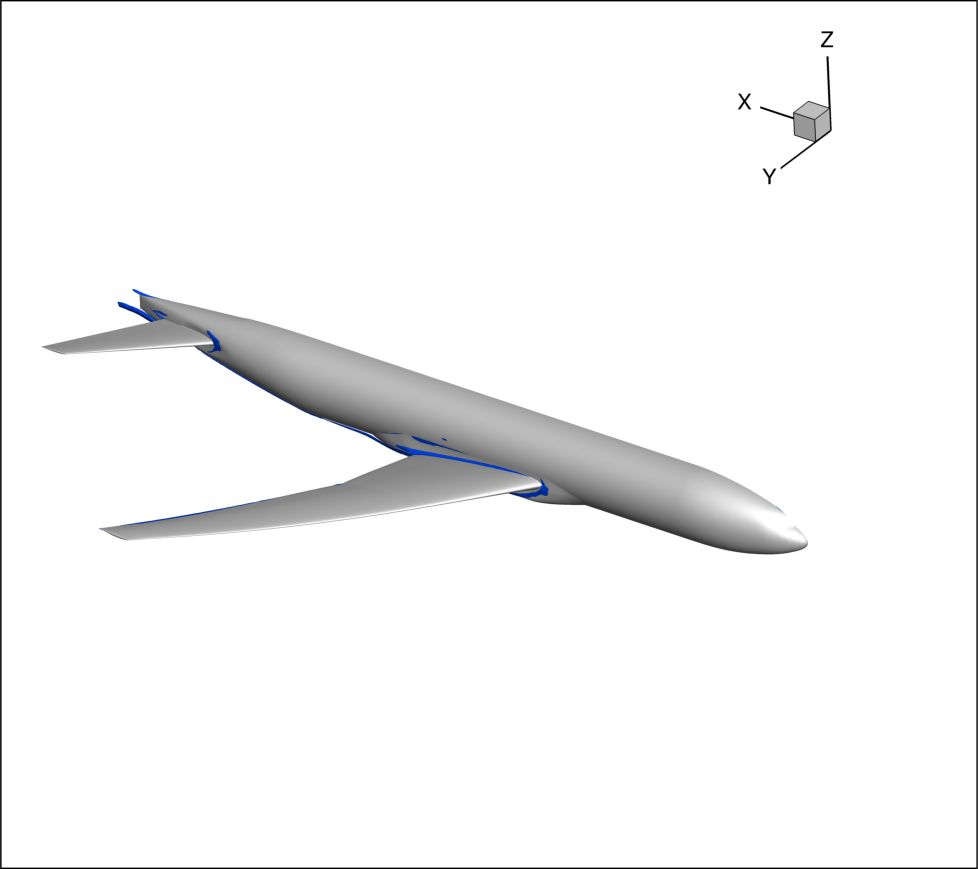
\includegraphics[trim=40 300 150 280, clip, width=.45\textwidth]{images/01aoa_mach02_isosurface.png} }
    \end{subfigure} 
    \hfill
    \begin{subfigure}[$\alpha = 2.35^\circ$.]{
        \label{fig:02aoa}
        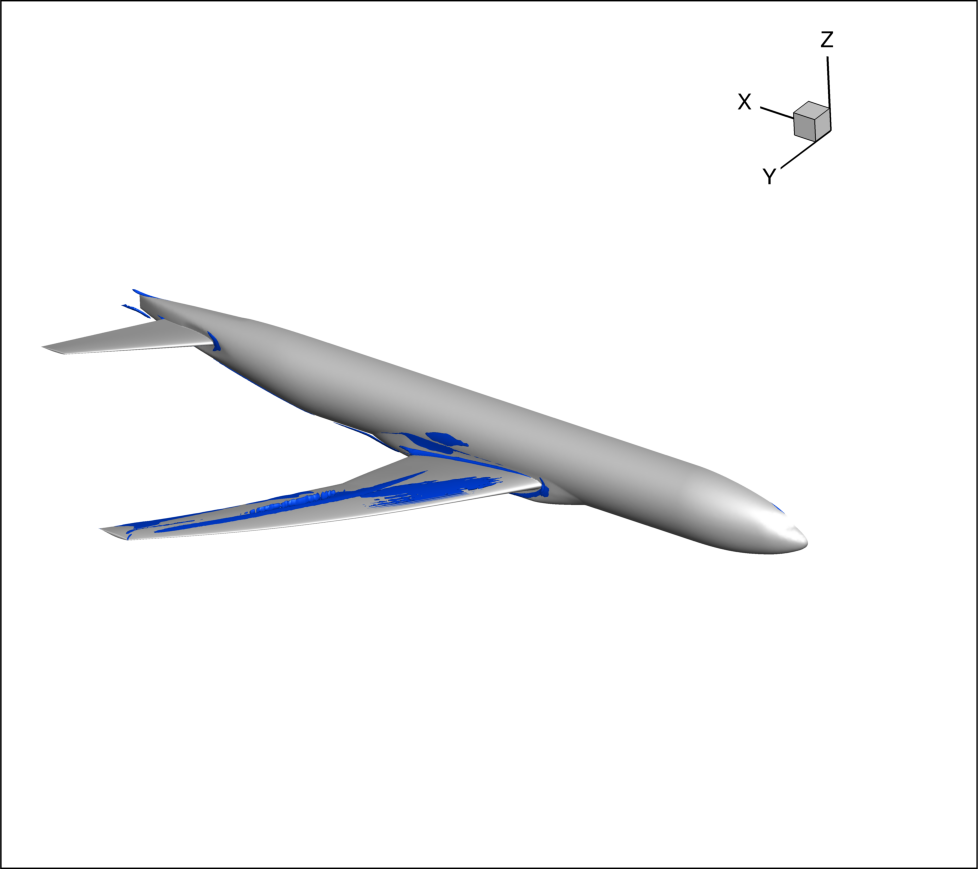
\includegraphics[trim=40 300 150 280, clip, width=.45\textwidth]{images/02_35381aoa_mach02_isosurface.png} 
    }
    \end{subfigure}
    \hfill
    \begin{subfigure}[$\alpha = 3^\circ$.]{
        \label{fig:03aoa}
        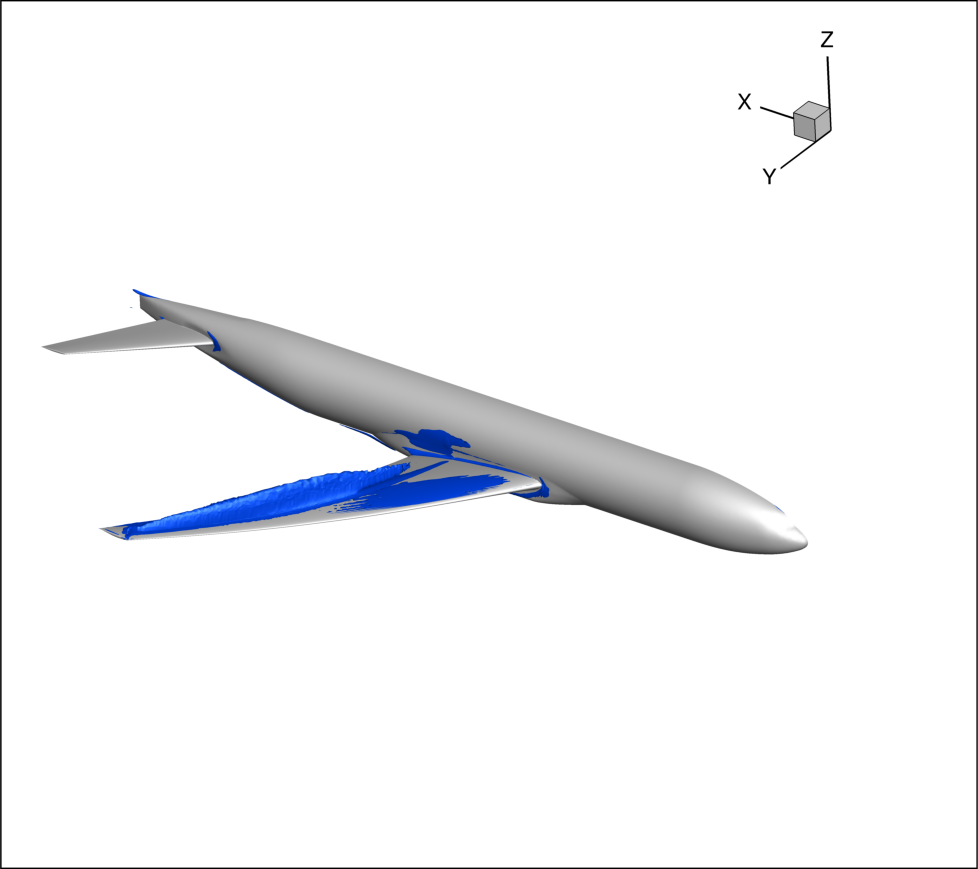
\includegraphics[trim=40 300 150 280, clip, width=.45\textwidth]{images/03aoa_mach02_isosurface.png} 
    }
    \end{subfigure}
    \hfill
    \begin{subfigure}[$\alpha = 4^\circ$.]{
        \label{fig:04aoa}
        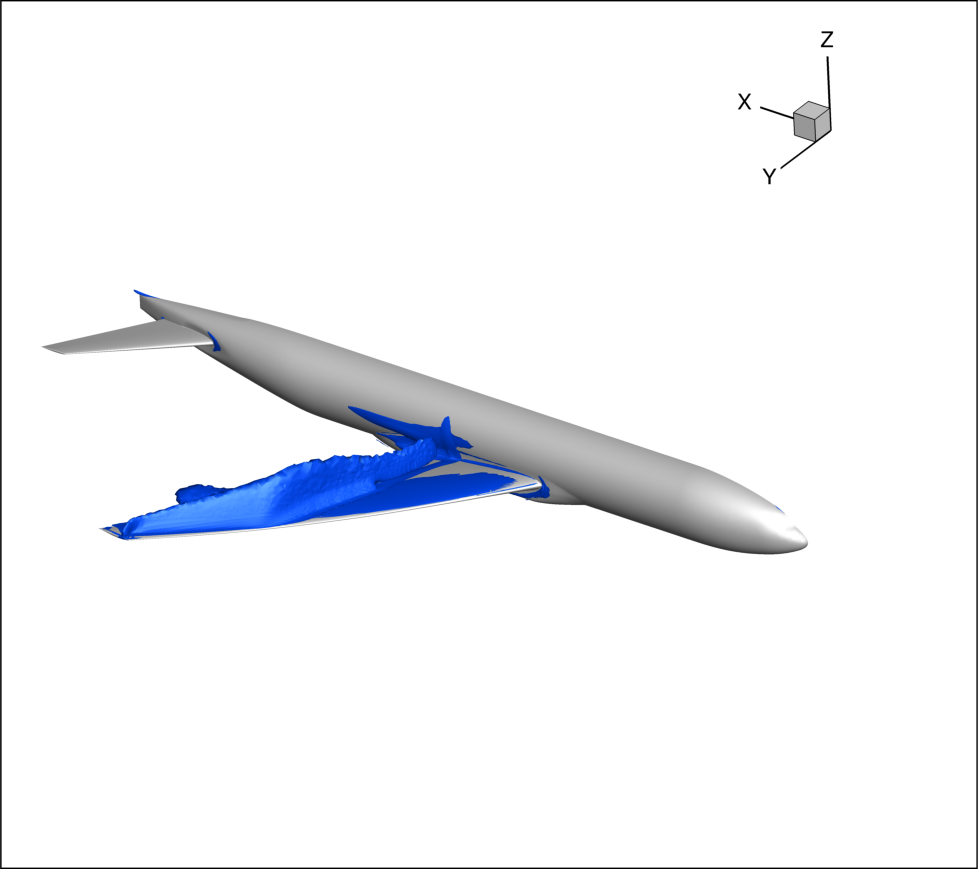
\includegraphics[trim=40 300 150 280, clip, width=.45\textwidth]{images/04aoa_mach02_isosurface.png} 
    }
    \end{subfigure}
    \hfill
    \caption{Isosurfaces representing areas where local Mach variability $M_v = 0.2$ at various angles of attack. \label{fig:mach_isosurface}}
\end{figure}

Similarly, the variability in any other flow quantity can be analyzed. Knowing which areas contribute to the uncertainty in performance predictions can aid design decisions. These results can inform sensor placement when moving to experimental campaigns. For example, a higher density of pressure sensors can be used in areas with large coefficient of pressure ($C_P$) variability. Flow visualization techniques can be focused on areas with large velocity variability. From the perspective of turbulence modeling, these variability visualizations can shed light on the types of flow features that are hard to predict with turbulence models. This additional data processing provides more qualitative applications for the RANS UQ methodology. 

\section{Fusion of multi-fidelity data} \label{sec:mf_fusion}

To provide more quantitative applications of the RANS UQ methodology, we demonstrate its inclusion in the multi-fidelity GP framework. To showcase the predictive capabilities of the multi-fidelity GP framework, the CFD data is augmented with both low-fidelity simulations, using the Athena Vortex Lattice (AVL) code \cite{drela2008athena}, and high-fidelity experimental data, from the wind tunnel campaigns \cite{rivers_further_2012,rivers_experimental_2010} used in the preceding section. For the vortex-lattice simulations, the uncertainty information is provided by subject matter experts (industry users and academics), while for the experimental data, the uncertainty intervals used are those described in the wind-tunnel campaign reports. 

For the ease of illustration, $C_L$, $C_D$, and $C_m$ are initially considered one-dimensional functions of $\alpha$ ($m = 1$). The methodology described in Section \ref{sec:mf_modeling} is generally applicable to functions of many variables. Aerodynamic databases are often multi-dimensional functions, often with a maximum of 5 input variables (angle of attack, side-slip angle, Mach number, altitude, and dynamic pressure). Multi-dimensional, multi-fidelity databases are explored towards the end of this section. 

The results of the multi-fidelity modeling with one input variable ($\alpha$) are presented in Figures \ref{fig:cl_alpha_mf} -- \ref{fig:cm_alpha_mf}. For each figure, the solid black line represents the mean predicted by the GP and the grey area represents the $\pm 2\sigma$ interval as predicted by the GP. The left column of figures shows purely the AVL data and a single-fidelity GP fit on that data. In the middle we introduce the SU2 RANS CFD data with uncertainty bounds informed by the RANS UQ methodology, and show the two-fidelity GP fit. On the right we introduce a limited set of wind tunnel data points to inform the highest fidelity, and show the resulting three-fidelity fit. For each QoI the build-up of the database is shown, and the distribution of data points across fidelity levels is shown in Table \ref{table:data_points}.

\begin{table}
\centering
    \captionsetup{justification=centering}
    \caption{Number of data points of each fidelity that are used to create Figures \ref{fig:cl_alpha_mf}-\ref{fig:cm_alpha_mf}.} 
    \begin{tabular}{|c|c|}
        \hline
        Data Source & Data Points \\ \hline \hline
        Low Fidelity (AVL) & 23 \\ \hline
        Medium Fidelity (CFD) & 11 \\ \hline 
        High Fidelity (Wind Tunnel) & 5 \\ \hline 
    \end{tabular}
    \label{table:data_points}
\end{table}

In the three-fidelity fits of Figures \ref{fig:cl_alpha_mf}(c) -- \ref{fig:cm_alpha_mf}(c) the wind tunnel data points are evenly spread across the domain of interest, $-2^\circ \leq \alpha \leq 12^\circ$. These data points also have uncertainties associated with them, but these are very small and cannot be seen on this scale in the figures. For the second and third column of figures, the mean and standard deviation predictions are made by the multi-fidelity GP methodology from Section \ref{sec:MF_GP}. 

\begin{figure}
    \centering
    \begin{subfigure}[Single fidelity fit.] {
        \includegraphics[width=.31\textwidth]{images/cl_1f.eps} }
    \end{subfigure}
    \hfill
    \begin{subfigure}[Two-fidelity fit.]{
        \includegraphics[width=.31\textwidth]{images/cl_2f.eps} 
    }
    \end{subfigure}
    \hfill
    \begin{subfigure}[Three-fidelity fit.]{
        \includegraphics[width=.31\textwidth]{images/cl_3f.eps} 
    }
    \end{subfigure}
    \caption{$C_L$ vs $\alpha$ for the NASA CRM, using data from multiple sources of varying fidelity.\label{fig:cl_alpha_mf}}
    \hfill
    \centering
    \begin{subfigure}[Single fidelity fit.] {
        \includegraphics[width=.31\textwidth]{images/cd_1f.eps} }
    \end{subfigure}
    \hfill
    \begin{subfigure}[Two-fidelity fit.]{
        \includegraphics[width=.31\textwidth]{images/cd_2f.eps} 
    }
    \end{subfigure}
    \hfill
    \begin{subfigure}[Three-fidelity fit.]{
        \includegraphics[width=.31\textwidth]{images/cd_3f.eps} 
    }
    \end{subfigure}
    \caption{$C_D$ vs $\alpha$ for the NASA CRM, using data from multiple sources of varying fidelity.\label{fig:cd_alpha_mf}}
    \hfill
    \centering
    \begin{subfigure}[Single fidelity fit.] {
        \includegraphics[width=.31\textwidth]{images/cm_1f.eps} }
    \end{subfigure}
    \hfill
    \begin{subfigure}[Two-fidelity fit.]{
        \includegraphics[width=.31\textwidth]{images/cm_2f.eps} 
    }
    \end{subfigure}
    \hfill
    \begin{subfigure}[Three-fidelity fit.]{
        \includegraphics[width=.31\textwidth]{images/cm_3f.eps} 
    }
    \end{subfigure}
    \caption{$C_m$ vs $\alpha$ for the NASA CRM, using data from multiple sources of varying fidelity.\label{fig:cm_alpha_mf}}
\end{figure}

The multi-fidelity GPs are able to learn the biases between the different fidelity levels and provide predictions that fit very well with the highest fidelity. To show the benefit of using multi-fidelity data vs. using only high-fidelity data points, the root-mean-square error (RMSE) for both cases and for each QoI is presented in Figure \ref{fig:mf_vs_hf}. The error is calculated using the $N$ highest-fidelity data points that aren't used in training the model as:

\begin{equation}\label{equ:rmse}
    RMSE = \sqrt{\frac{\sum_{i=1}^{N}\left ( \mu_{s,i} - y_{s,i} \right )^2}{N}},
\end{equation}
where $y_{s,i}$ is the $i$-th data point of the highest ($s$) fidelity, and $\mu_{s,i}$ is the highest-fidelity prediction from the GP at the same input conditions.  

Since the QoIs are simple functions of $\alpha$, not many high-fidelity data points are required to accurately capture the functional dependence. The differences between the prediction accuracy for a single- vs. multi-fidelity fit is not significant. Nonetheless, the trends are what would be expected. When high-fidelity data is scarce, the multi-fidelity predictions perform better for all QoIs since the low-fidelity data helps provide general trends that are learned by the multi-fidelity GP. As the number of high-fidelity data points increases, the RMSEs converge since there is enough data for both fits to accurately reproduce the functional dependence. When the domain is very well covered by high-fidelity data, the single-fidelity fits can do marginally better since the low-fidelity data (in the multi-fidelity fits) doesn't provide any useful information and can serve to introduce noise in the predictions.

\begin{figure}
    \centering
    \begin{subfigure}[RMSE for $C_L$ vs. $\alpha$.] {
        \includegraphics[width=.31\textwidth]{images/cl_rsme_comp.eps} }
    \end{subfigure}
    \hfill
    \begin{subfigure}[RMSE for $C_D$ vs. $\alpha$.]{
        \includegraphics[width=.31\textwidth]{images/cd_rsme_comp.eps} 
    }
    \end{subfigure}
    \hfill
    \begin{subfigure}[RMSE for $C_m$ vs. $\alpha$.]{
        \includegraphics[width=.31\textwidth]{images/cm_rsme_comp.eps} 
    }
    \end{subfigure}
    \caption{Root Mean Square error when using three-fidelity data vs. using only high-fidelity data points.\label{fig:mf_vs_hf}}
\end{figure}

Another strength of this multi-fidelity GP methodology is apparent when the high-fidelity data is localized to a certain part of the domain. Such a situation might arise if resources are limited and it is not feasible to perform high-fidelity evaluations over the entire domain of interest. It might also be the case that the lower-fidelity simulations are fairly accurate in a certain part of the domain and, consequently, introduce smaller uncertainties in these regions of the domain. For the NASA CRM it is mentioned in Section \ref{sec:crm_uq} that at low angles of attack, where the flow remains attached to the aircraft, RANS CFD simulations are quite successful at predicting performance metrics. This is evidenced by the smaller uncertainty bounds predicted by the RANS UQ methodology in Figure \ref{fig:crm_su2_uq} at $\alpha < 5^\circ$. In this case, an engineer might conclude that highest-fidelity evaluations are not necessary at $\alpha < 5^\circ$ and that sufficient accuracy can be achieved with just the lower-fidelity sources. 

To simulate such a situation, a multi-fidelity GP is created that uses AVL and SU2 data that spans the entire domain of interest, but uses wind tunnel evaluations only at high angles of attack $(\alpha > 5^\circ)$. This is a manufactured situation where we choose to ignore some of the wind tunnel data to illustrate the ability of the multi-fidelity GP framework to perform reliably without high-fidelity information that spans the domain of interest. Figure \ref{fig:mf_partial} presents the predictions made by a three-fidelity GP trained on AVL, SU2, and wind tunnel data (left column), and a single-fidelity GP trained on just the wind tunnel data (middle column). The wind tunnel data used to train the models is restricted to high angles of attack, but the unused wind tunnel data is also included in the plots to discern the quality of the predictions. The right column presents the RMSE of the predictions made by the single- and multi-fidelity GPs when using localized high-fidelity data. The case that is shown in the left and middle columns, is highlighted in this error comparison. From the RMSE comparison, it is clear that having accurate low-fidelity data at low angles of attack informs the GP prediction in that region, and allows it to follow the trend of the physical phenomena more accurately than when only the localized high-fidelity data is used. 

\begin{figure}
    \centering
    \begin{subfigure}[$C_L vs. \alpha$: Three-fidelity fit.] {
        \includegraphics[width=.31\textwidth]{images/cl_3f_partial.eps} }
    \end{subfigure}
    \begin{subfigure}[$C_L vs. \alpha$: Single fidelity fit.]{
        \includegraphics[width=.31\textwidth]{images/cl_hf_partial.eps} 
    }
    \end{subfigure}
    \hfill
    \begin{subfigure}[$C_L vs. \alpha$: RMSE trends when data is added sequentially from high to low values of $\alpha$.]{
        \includegraphics[width=.31\textwidth]{images/cl_rsme_local_comp.eps} 
    }
    \end{subfigure}

    \begin{subfigure}[$C_D vs. \alpha$: Three-fidelity fit.] {
        \includegraphics[width=.31\textwidth]{images/cd_3f_partial.eps} }
    \end{subfigure}
    \begin{subfigure}[$C_D vs. \alpha$: Single fidelity fit.]{
        \includegraphics[width=.31\textwidth]{images/cd_hf_partial.eps} 
    }
    \end{subfigure}
    \hfill
    \begin{subfigure}[$C_D vs. \alpha$: RMSE trends when data is added sequentially from high to low values of $\alpha$.]{
        \includegraphics[width=.31\textwidth]{images/cd_rsme_local_comp.eps} 
    }
    \end{subfigure}

    \begin{subfigure}[$C_m vs. \alpha$: Three-fidelity fit.] {
        \includegraphics[width=.31\textwidth]{images/cm_3f_partial.eps} }
    \end{subfigure}
    \begin{subfigure}[$C_m vs. \alpha$: Single fidelity fit.]{
        \includegraphics[width=.31\textwidth]{images/cm_hf_partial.eps} 
    }
    \end{subfigure}
    \hfill
    \begin{subfigure}[$C_m vs. \alpha$: RMSE trends when data is added sequentially from high to low values of $\alpha$.]{
        \includegraphics[width=.31\textwidth]{images/cm_rsme_local_comp.eps} 
    }
    \end{subfigure}
    
    \caption{Showcasing the superior predictive capability of multi-fidelity data fusion when high-fidelity data is localized in the design space. The left column represents the multi-fidelity GP formulation result, while the middle column shows the results for the single-fidelity formulation. The right column shows the RMSE error trends when high-fidelity data is localized. The black circles correspond to the specific case shown in the left and middle columns. \label{fig:mf_partial}}
    
\end{figure}

To explore the performance of the multi-fidelity predictive capability in multiple dimensions, the same aerodynamic coefficients from before ($C_L$, $C_D$, and $C_m$) are considered functions of both $\alpha$ and Mach number. Two sources of information, AVL simulations and wind tunnel data, are used to create two-fidelity, two-dimensional GPs. Visualizing the GP predictions in two dimensions is difficult but the results for $C_L$ are shown in Figure \ref{fig:2d_2f_cl_data}. Figure \ref{fig:cl_2d_2f_points} shows the two-fidelity data sets that are used to train the multi-fidelity GP. Figure \ref{fig:cl_2d_2f_surf} shows the surfaces that represent the mean (as a contoured solid surface), and $2\sigma$ interval estimates (as translucent surfaces sandwiching the mean prediction). The difference between the mean and intervals is hard to discern at that scale. Figure \ref{fig:cl_2d_2f_surf_zoom} focuses in on the high-angle of attack (and low Mach number) area when the uncertainties are larger, to show the different surfaces clearly. To show a one-dimensional representation of the data, a slice spanning the two dimensions is taken (shown in red). The mean and $2\sigma$ intervals along that slice are plotted in Figure \ref{fig:cl_2d_2f_sample}, along with some deterministic samples of the GP (multi-colored lines) that show how they might vary spatially. Again since uncertainties are small, an inset focuses on the high-angle of attack (and low Mach number) area of the domain where the individual samples can be recognized.

\begin{figure}
    \centering
    \begin{subfigure}[AVL and wind tunnel data points.] {
        \label{fig:cl_2d_2f_points}
        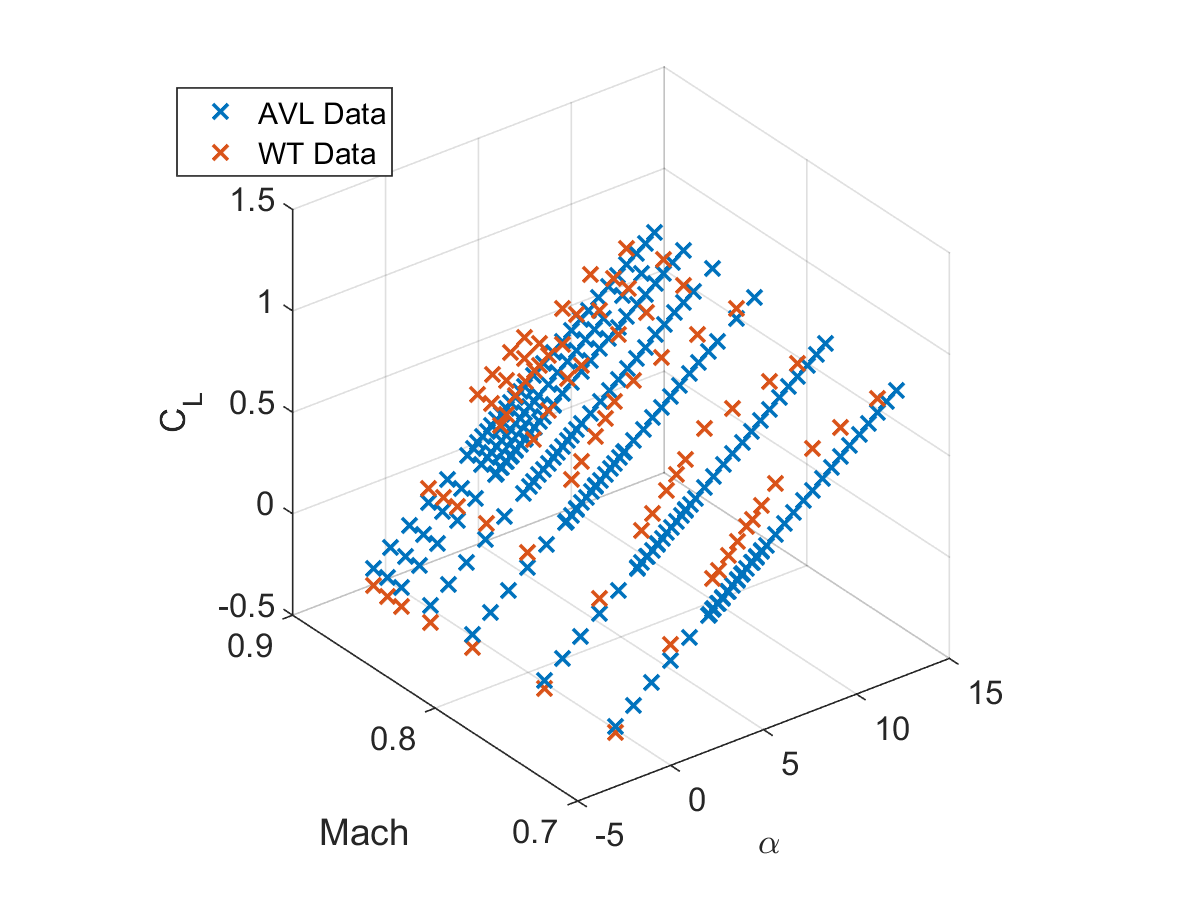
\includegraphics[trim=70 10 90 20, clip, width=.45\textwidth]{images/cl_2d_2f_points.png} }
    \end{subfigure}
    \hfill
    \begin{subfigure}[Surfaces representing mean and $2\sigma$ predictions from GP. Red slice shows one-dimensional location for sampling the GP which is shown in \subref{fig:cl_2d_2f_sample}.]{
        \label{fig:cl_2d_2f_surf}
        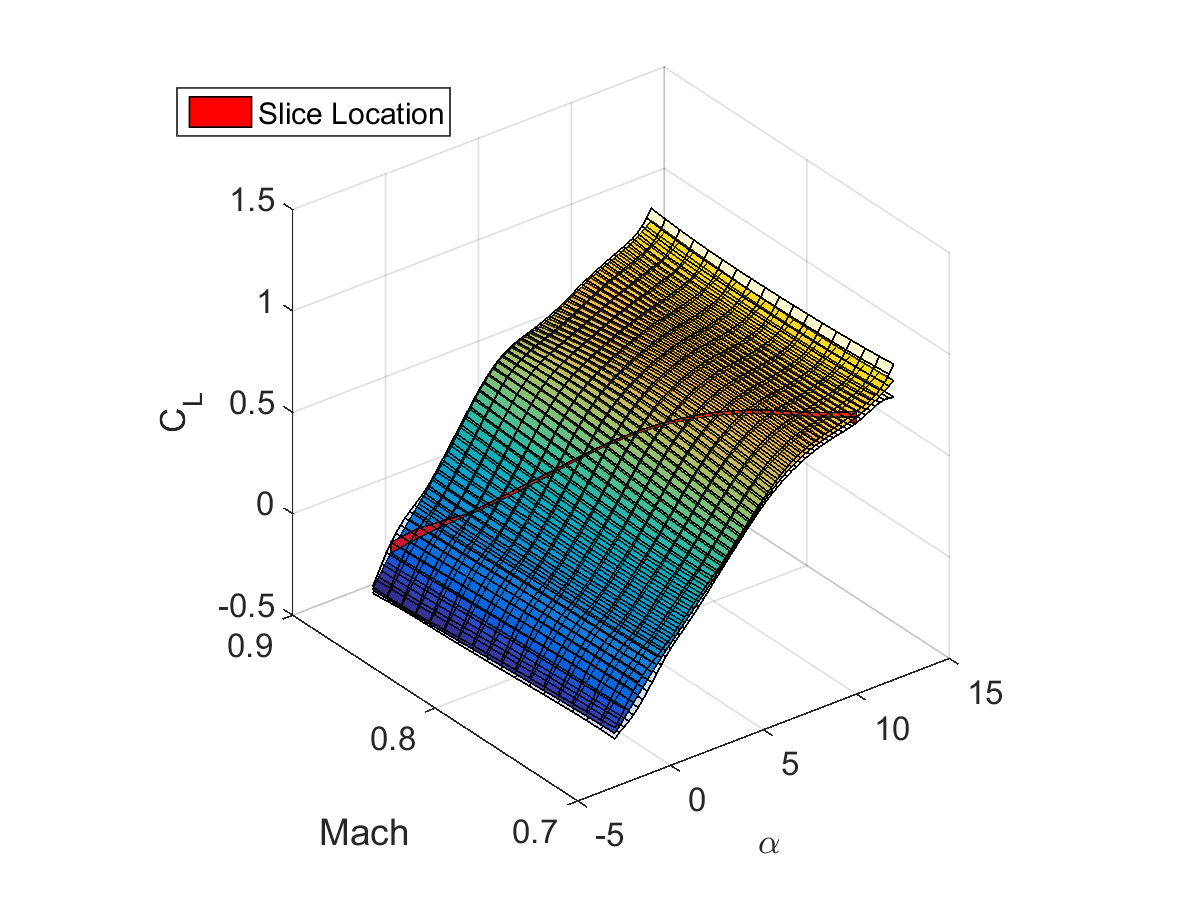
\includegraphics[trim=70 10 90 20, clip, width=.45\textwidth]{images/cl_2d_2f_surf.png} 
    }
    \end{subfigure}
    \hfill
    \begin{subfigure}[Zoomed in view of surfaces in \subref{fig:cl_2d_2f_surf} at high angles of attack (and lower Mach number). The mean and $2\sigma$ predictions interval surfaces are more discernible at this scale.]{
        \label{fig:cl_2d_2f_surf_zoom}
        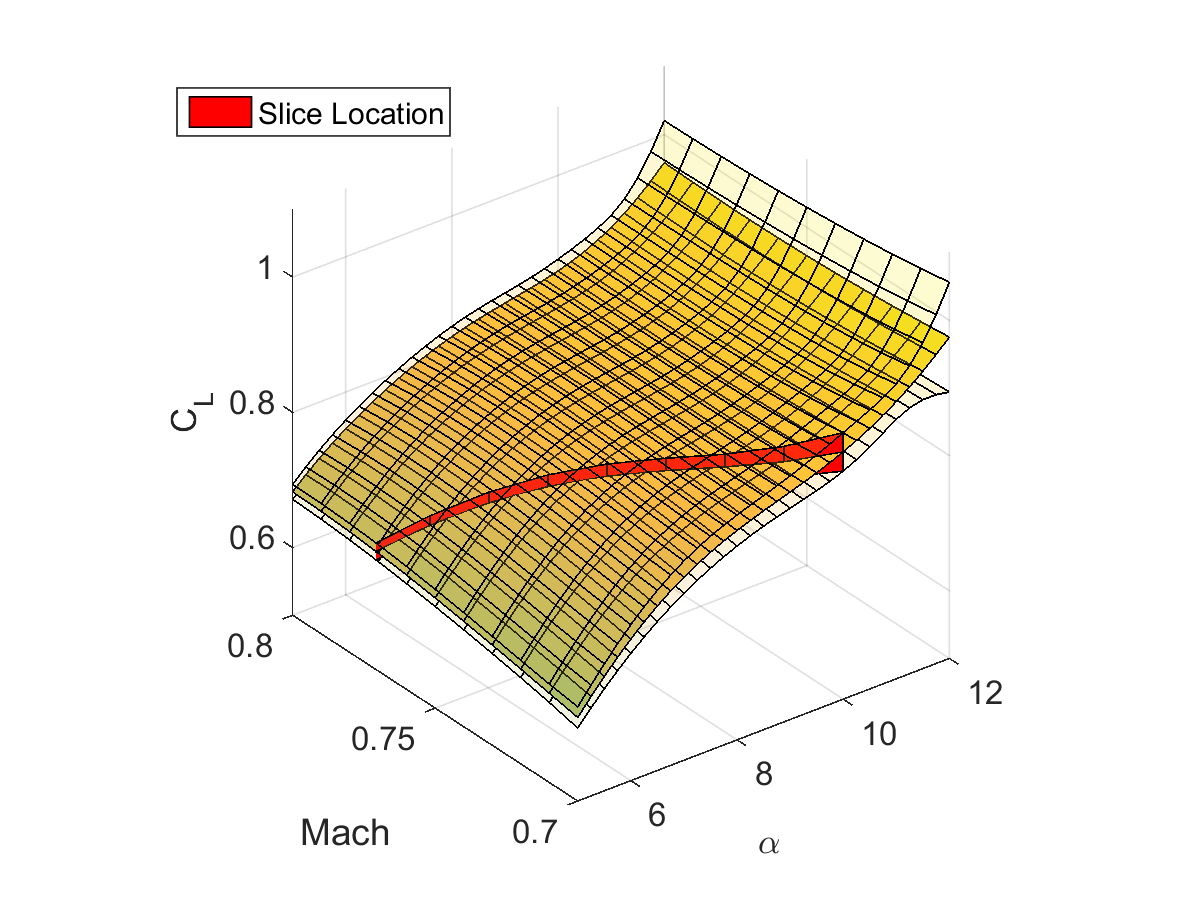
\includegraphics[trim=70 10 90 20, clip, width=.45\textwidth]{images/cl_2d_2f_surf_zoom.png} 
    }
    \end{subfigure}
    \hfill
    \begin{subfigure}[One-dimensional representation of mean and $2\sigma$ estimates at slice location shown in \subref{fig:cl_2d_2f_surf}. Multiple samples (colored lines) of the GP are also overlaid to show examples of deterministic sampling. Inset plot focuses in on high angles of attack.]{
        \label{fig:cl_2d_2f_sample}
        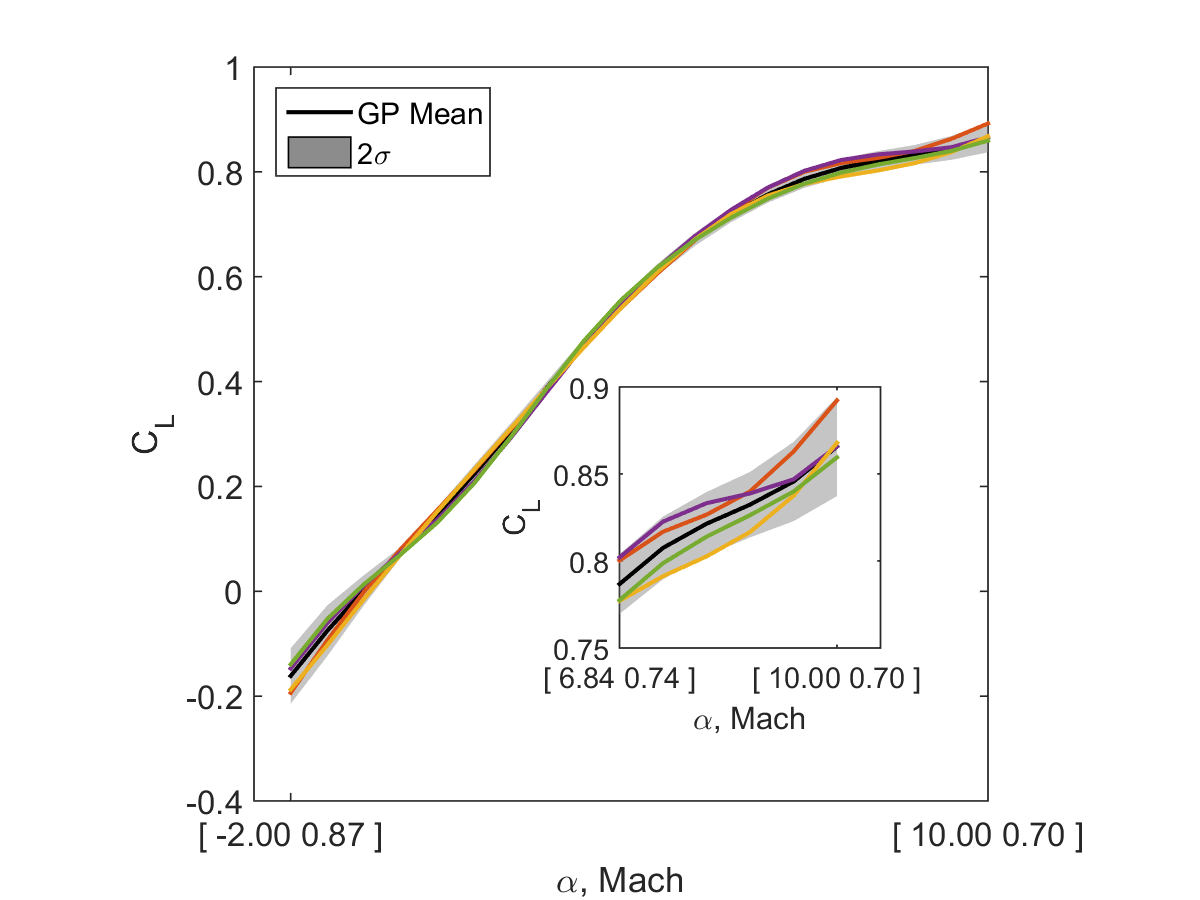
\includegraphics[trim=60 0 50 20, clip, width=.45\textwidth]{images/cl_2d_2f_sample.png} 
    }
    \end{subfigure}
    \caption{Two-dimensional representation of $C_L$ as a function of $\alpha$ and Mach number.\label{fig:2d_2f_cl_data}}
\end{figure}

Predictions from the two-fidelity GPs are compared to those made from single-fidelity GPs that use only the wind tunnel data. The change in the root-mean-square-error (Equation \eqref{equ:rmse}) is shown in Fig \ref{fig:2d_mf_vs_hf}. When trying to represent two-dimensional functions, the multi-fidelity fit retains its advantage for longer, with the single-fidelity fit taking $\approx 50$ high-fidelity data points to achieve similar accuracy. If the number of high-fidelity points is increased beyond that, the two fits behave identically. For these results, the high-fidelity data was spread evenly across the domain of interest: $-2^\circ \leq \alpha \leq 12^\circ$ and $0.7 \leq \text{Mach} \leq 0.87$. As the number of input dimensions is increased, more data points would be required to capture the functional trends. Leveraging the multi-fidelity improvement in these high-dimensional spaces would be beneficial in reducing time spent collecting high-fidelity data where a lower-fidelity might suffice.

\begin{figure}
    \centering
    \begin{subfigure}[RMSE for $C_L$.] {
        \includegraphics[width=.31\textwidth]{images/cl_2d_rsme_lhs_comp.eps} }
    \end{subfigure}
    \hfill
    \begin{subfigure}[RMSE for $C_D$.]{
        \includegraphics[width=.31\textwidth]{images/cd_2d_rsme_lhs_comp.eps} 
    }
    \end{subfigure}
    \hfill
    \begin{subfigure}[RMSE for $C_m$.]{
        \includegraphics[width=.31\textwidth]{images/cm_2d_rsme_lhs_comp.eps} 
    }
    \end{subfigure}
    \caption{Root-mean-square-error for two-dimensional functions of Mach and $\alpha$ when using two-fidelity data vs. using only high-fidelity data points.\label{fig:2d_mf_vs_hf}}
\end{figure}
